\documentclass{emulateapj}
\bibliographystyle{astroads}

%define general packages
\usepackage{epsfig}
\usepackage{amsmath}
\usepackage{natbib}
\usepackage{afterpage}
\usepackage{xcolor}
\newcommand\writingnote[1]{\textcolor{red}{#1}}
% \renewcommand\writingnote[1]{}
% \renewcommand\actpol[1]{}
\newcommand{\LCDM}   {$\Lambda$CDM}
\newcommand{\planck}{{\it Planck}}
\newcommand{\wmap}{{\it WMAP}}
\newcommand  \be    {\begin{equation}}
\newcommand  \ee    {\end{equation}}
\newcommand{\ba}{\begin{eqnarray}}
\newcommand{\ea}{\end{eqnarray}}


\DeclareMathAlphabet\mathbfcal{OMS}{cmsy}{b}{n}
\newcommand{\prr}{ \mathcal{P}_{\mathcal{R}\mathcal{R}} }
\newcommand{\pri}{ \mathcal{P}_{\mathcal{R}\mathcal{I}} }
\newcommand{\pii}{ \mathcal{P}_{\mathcal{I}\mathcal{I}} }


\begin{document}

\title{Future constraints on isocurvature fluctuations from the Cosmic Microwave Background}
\author{Zack Li and Jo Dunkley}
\date{\today}
%\maketitle
\affil{Astrophysical Sciences, Princeton University, Princeton NJ 08544}


\begin{abstract}
We provide forecasts of cold dark matter isocurvature (CDI) constraints for combinations of Planck, CMB S4, and PIXIE. Using MCMC methods on fiducial power spectra, we find substantial improvements in the measurement of the large scale isocurvature power.
\end{abstract}

%Section heading
\section{Introduction}

Current cosmological data support the standard `\LCDM' cosmological model, a flat universe with primordial fluctuations that are scalar, adiabatic, and Gaussian, and are described by a power spectrum with an amplitude and power-law spectral index \citep{planckXX:2015}. The adiabatic nature of the fluctuations come from a spatially uniform equation of state and initial velocity field and lock together the density perturbations of the different components \citep{planckXXII:2013}. The physical origin of the primordial fluctuations is still not known however, and the most general perturbations include not only adiabatic fluctuations, but also isocurvature perturbations, with spatially varying equations of state or initial velocity fields \citep{adiab}. A non-zero level of isocurvature fluctuations is still allowed by current data.

Isocurvature fluctuations can take the form of variations between the photon and the cold dark matter (CDM) density, the photon and baryon density, or the photon and neutrino density \citep{moodley/bucher/turok:2000}. Variations between the photon velocity and neutrino velocity are also possible. Within an inflation scenario with a single scalar field and slow-roll initial conditions, only adiabatic perturbations are expected. However, isocurvature fluctuations could be generated from a variety of physical scenarios including multiple field inflation \citep{langlois:1999}, and the curvaton scenario
%which generates CDM isocurvature perturbations correlated with the adiabatic modes
\citep{baumann/etal:2009}. Some string theory axions can also generate isocurvature fluctuations from quantum fluctuations, with axion decay to dark matter leading to uncorrelated adiabatic and CDM isocurvature perturbations \cite{axion}. (Mention compensated isocurvature). Early universe models other than inflation could also generate isocurvature.

Data from the \wmap\ satellite, supplemented by Baryon Acoustic Oscillation data, have been used to put upper bounds on the fractional contribution of CDI to the primordial power at less than a percent \citep{hinshaw/etal:2013}, assuming a fixed power-law index and considering either fully uncorrelated or anticorrelated modes. This CDI mode is considered the most physically well-motivated, and is observationally equivalent to baryon isocurvature. Combinations of different isocurvature modes were allowed at a much higher degree \cite{bean}. The \planck\ data reduce the limits on fully correlated power-law CDI to XX, and for a more general partially correlated model limit the fractional power  to be less than 2\% at large scales ($k=0.002$ Mpc$^{-1}$), and less than 52\% at smaller scales ($k=0.1$ Mpc$^{-1}$ \citep{planckXX:2015}. 
%These use polarization measurements over the Planck range of $l=2-2508$ for TT and $2-1996$ for TE and EE.

There is still scope for improvement. The isocurvature temperature and polarization power spectra are out of phase with the adiabatic perturbations, so improved CMB polarization measurements can considerably tighten constraints. We find that currently available ground-based polarization data from the Atacama Cosmology Telescope improve constraints over \planck\ by of order 10\%, but expect the completed CMB Stage-3 and Stage-4 experiments to provide much greater gains. CMB-S4 is a next-generation ground-based CMB experiment planned for observations in the 2020s, involving hundred of thousands of detectors. It will reduce the polarization noise levels over \planck\ by almost a factor of one hundred, reaching to small angular scales. Proposed low-resolution satellites including PIXIE and LiteBIRD will offer similar improvement for larger angular scales \citep{pixie,litebird}. Forecasts for CMB-S4  predict an increase in sensitivity by a factor of 3-6 over \planck\ for the curvaton scenario \citep{CMB-S4:2016}. \cite{kasanda/moodley:2014} forecast the capabilities of a future CMB satellite, and \cite{smith/grin:2016} forecast that a cosmic-variance limited experiment could reach XX. 
%and investigate the effects of the CMB lensing potential.

In this paper we explore how well the degree of CDI can be constrained with a CMB-S4 level experiment and the proposed PIXIE satellite.  Similar results would hold for the proposed LiteBIRD satellite. We consider the general CDI model explored by \citet{planck_inflation}, which allows partial correlation of modes and a variable spectral index. 
 %We improve upon these results by including an atmospheric model calibrated for the Atacama desert for CMB-S4, and choose a more general isocurvature model.  While we do not involve PRISM, we do explore combinations of Planck, S4, and PIXIE.
In Section \ref{methods}, we describe the effect of isocurvature on power spectra, our chosen parametrization, and the details of the experimental specifications used in the forecasts. In Section \ref{results}, we present our forecasted constraints, and discuss in section \ref{discussion}.
%we provide some conclusions about the science yield from each experiment and the whether future measurements will be able to differentiate between models for the origin of the primordial density fluctuations.  


\section{Methods}\label{methods}

\begin{figure}[h]
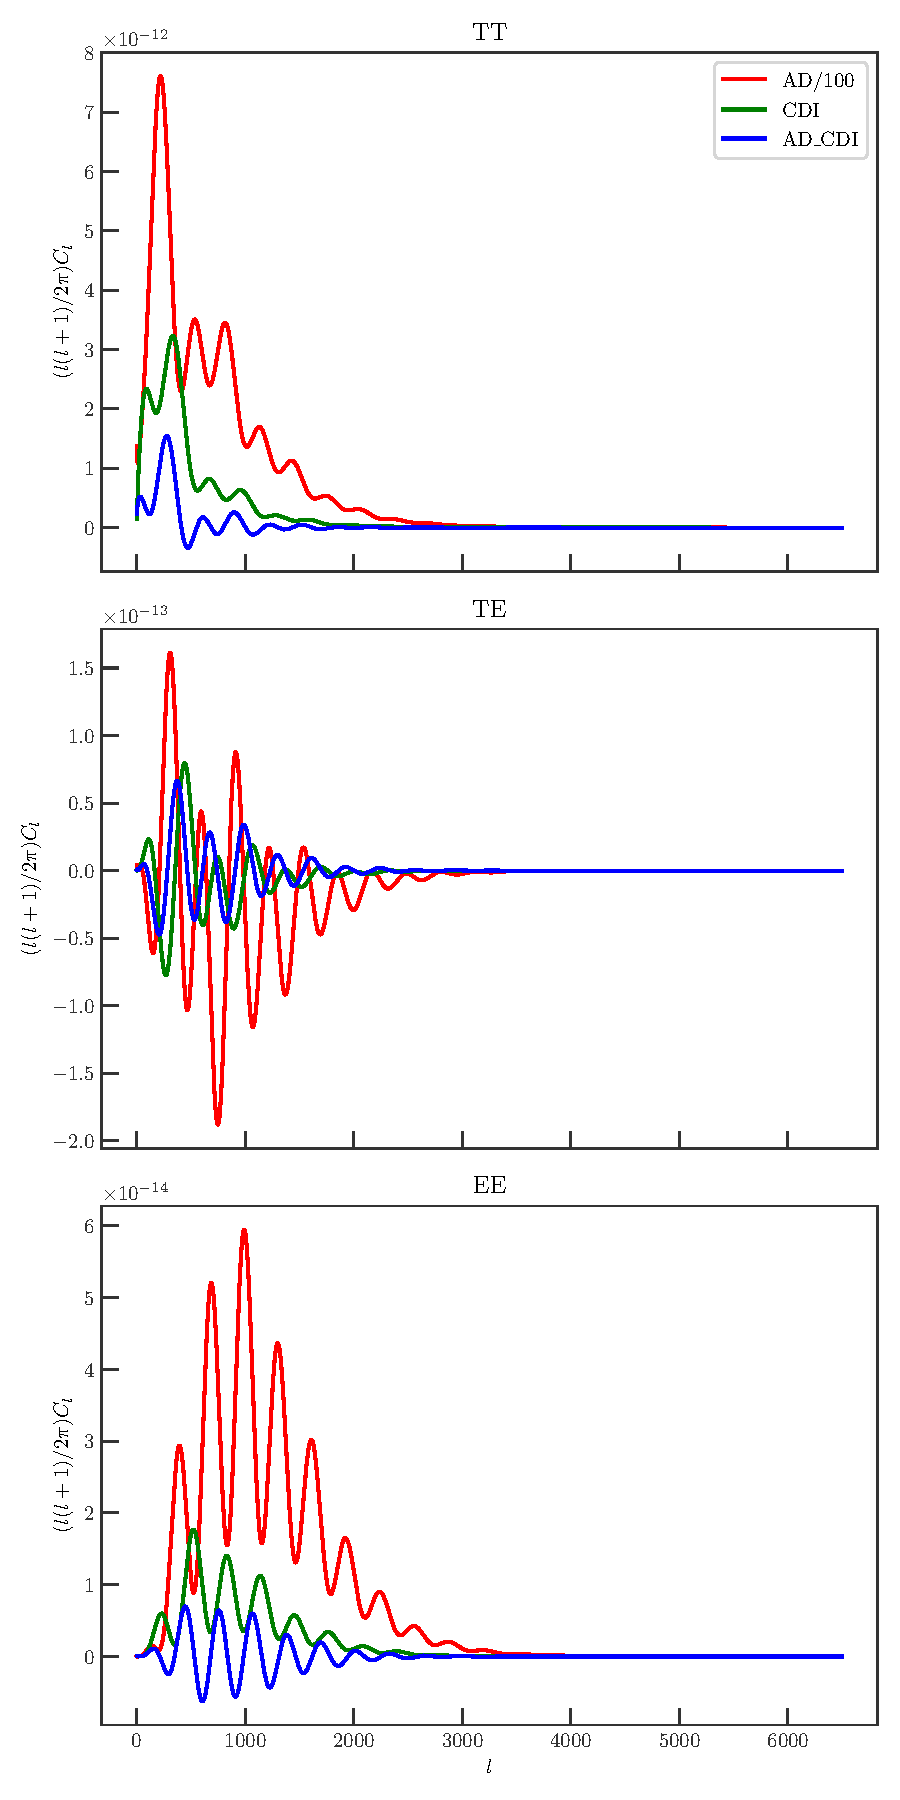
\includegraphics[width=0.45\textwidth]{figures/isocurvature_fiducial_spectra_contributions.pdf}
% \plotone{figures/isocurvature_fiducial_spectra_contributions.pdf}
\caption{Scaled adiabatic and isocurvature contributions to $\mathcal{D}_l$ for a model with nonzero isocurvature consistent with the Planck measurements. \writingnote{overplot ACTPol error bars, plot adiabatic normally and scale isocurvature contributions by 100}\label{fig:effects}}
\end{figure}


\subsection{Perturbations and Power Spectra}\label{powerspectra}

%\writingnote{
%todo: heuristic description of isocurvature effects on CMB power spectra. maybe I include something like the $dD_l/dP_{II}^j$ plots.
%}

Gaussian fluctuations for a general cosmological perturbation can be described by a matrix of their power spectra, including both auto- and cross-power spectra. In this paper we only consider primordial CDM isocurvature (CDI) and adiabatic modes, so the matrix describing their power is $2 \times 2$,  

\begin{equation}
\mathbfcal{P}(k) = \left( {\begin{array}{cc}
   \prr(k) & \pri(k) \\
   \pri(k) &  \pii(k) \\
  \end{array} } \right)
\end{equation}
Here, $\prr(k)$ is the power spectrum of curvature perturbations, and $\pii(k)$ is the power spectrum of $\delta \rho_{\rm CDM} / \rho_{\rm CDM}$, with $\rho_{CDM} = n_c / n_{\gamma}$, the ratio of primordial CDM to photon number densities {\bf (Jo- check this definition)}. $\pri(k)$ is the cross-spectrum.

Following \cite{planckXX:2015}, we parametrize $\prr$, $\pri$, and $\pii$ by defining the power at two scales, $k_1 = 0.002$ Mpc$^{-1}$ and $k_2 = 0.100$ Mpc$^{-1}$ and interpolating geometrically,
\begin{align*}
\mathcal{P}_{ab}(k) = & \exp \bigg[ \left( \frac{\ln(k) - \ln(k_2)}{\ln(k_1) - \ln(k_2)}\right) \ln \left( \mathcal{P}_{ab}^1 \right) \\
& +
\left( \frac{\ln(k) - \ln(k_1)}{\ln(k_2) - \ln(k_1)}\right) \ln \left( \mathcal{P}_{ab}^2 \right) \bigg].
\end{align*}
Thus the spectral index of each component is given by
\be n_{\text{ab}}  =  \frac{\log( \mathcal{P}_{\text{ab}}^2 / \mathcal{P}_{\text{ab}}^1 )}{\log ( k_2 / k_1 )}. \ee

We compute the theoretical lensed power spectra with CLASS, a fast Boltzmann code \citep{class}, with primordial amplitudes defined by five parameters, $\prr^{(1)}$, $\prr^{(2)}$,  $\pii^{(1)}$, $\pii^{(2)}$, and $\pri^{1}$. 
%The adiabatic and isocurvature are contained in three functions, $\mathcal{P}_{\mathcal{RR}}(k)$, $\mathcal{P}_{\mathcal{II}}(k)$, and $\mathcal{P}_{\mathcal{RI}}(k)$, the curvature, isocurvature, and cross-correlation power spectra, respectively (cite Planck 2015 XX).

%We use the same uniform priors as Planck,
%\begin{equation}
%    \prr^{(1)}, \prr^{(2)} \in (10^{-9}, 10^{-8}),
%\end{equation}
%\begin{equation}
%    \pii^{(1)}, \pii^{(2)} \in (0, 10^{-8}),
%\end{equation}
%\begin{equation}
%    \pri^{(1)} \in (-10^{-8}, 10^{-8}).
%\end{equation}
We follow the \planck\ convention of fixing $\pri^{(2)}$ by requiring the correlation fraction, $\Delta$, to be scale-independent. Here
\begin{equation}
\cos \Delta = \frac{\pri}{(\prr \pii)^{1/2}}, % \in (-1,1),
\end{equation}
so that
\begin{equation}
\pri^{(2)} = \pri^{(1)} \frac{\left(\prr^{(2)} \pii^{(2)} \right)^{1/2}}{ \left(\prr^{(1)} \pii^{(1)} \right)^{1/2}}.
\end{equation}



\begin{figure}
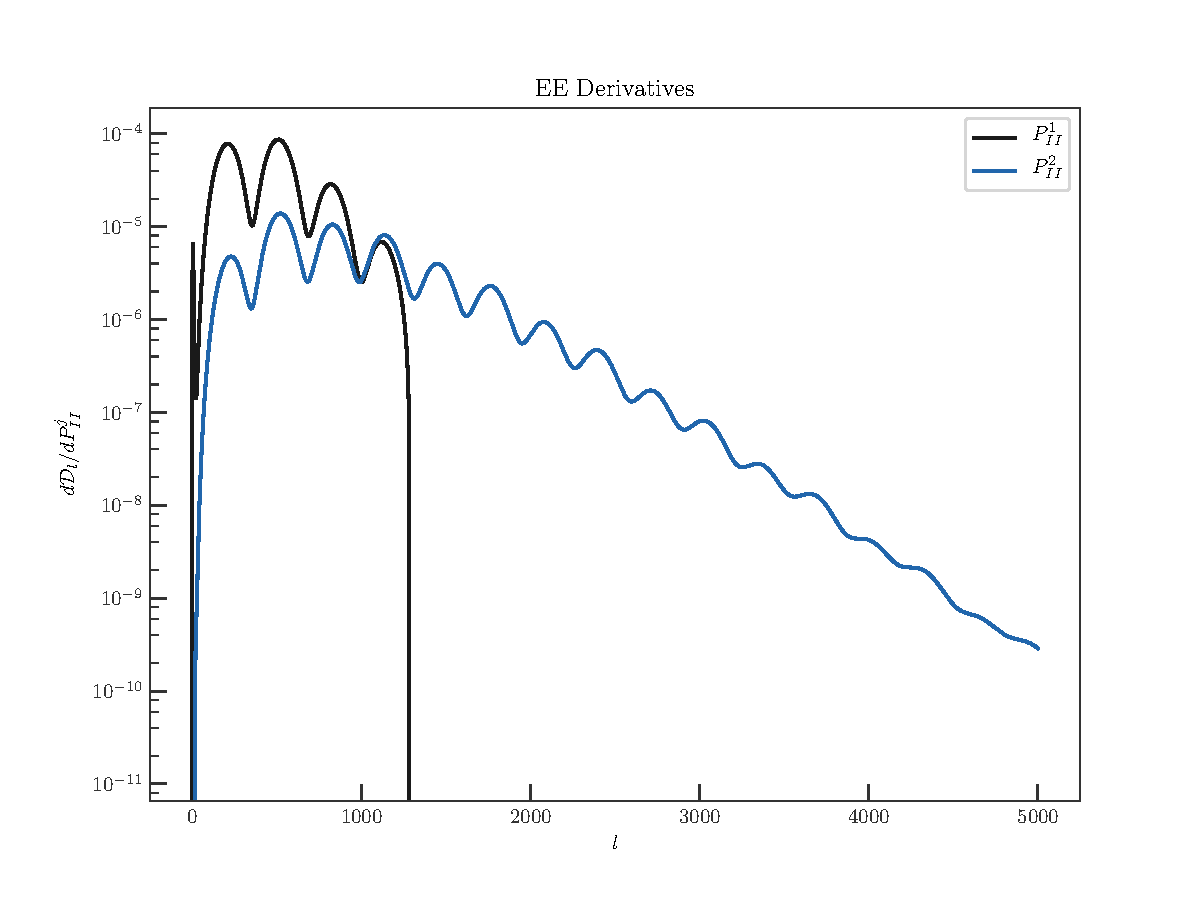
\includegraphics[width=0.5\textwidth]{figures/logee.pdf}
% \plotone{figures/isocurvature_fiducial_spectra_contributions.pdf}
\caption{A measurement of the impact of the two isocurvature powers $\pii^1$ and $\pii^2$, by taking the derivative of $\mathcal{D}_l$ with respect to $\pii^i$, for a model with nonzero isocurvature consistent with the Planck measurements.\label{fig:derivs}}
\end{figure}

\subsection{Forecasting}\label{forecasting}

In this analysis we choose to use an MCMC sampling method with simulated data, rather than a Fisher matrix approach, given the highly non-Gaussian nature of the parameter distributions.

We simulate CMB-S4 and PIXIE temperature and polarization likelihoods following \cite{perotto/etal:2006} using standard methods. We define a multipole range, sky fraction $f_{\text{sky}}$, beam size $\theta_{\text{fwhm}}$, temperature noise $\sigma_T$, and polarization noise $\sigma_P$. The noise properties, for $X,Y \in \{T, E, B\}$, are given by
\begin{equation}
\mathbf{N}_l^{XY} = \delta_{XY} \theta_{\text{fwhm}}^2 \sigma_X^2 \exp \left[  l(l+1) \frac{\theta_{\text{fwhm}}}{8 \ln 2}  \right].
\end{equation}
The errors on the power spectrum are computed using the Knox formula {\bf (what happens at low ell - we assume still Gaussian?)}. The instrumental parameters are given in Table \ref{table:forecasts}. We also simulate \planck\ data using the same method, to check our pipeline against the achieved \planck\ results {\bf (What is the low-ell likelihood)}. For CMB-S4, we test the inclusion of an atmospheric noise model, in the form of a fitting function with $\ell_{\text{knee}} = 330$, $\alpha = -3.8$ \citep{hasselfield},
\be
N_\ell = N_0 \left( 1 + \left(\frac{\ell}{\ell_{\text{knee}}}\right)^{\alpha} \right).
\ee


\begin{deluxetable*}{cccccc}
\label{table:forecasts}
\tabletypesize{\footnotesize}
\tablecolumns{6}
\tablewidth{0pt}
\tablecaption{ Forecasting Parameters }
\tablehead{
 \colhead{Experiment}     & \colhead{$l_{min}$ - $l_{max}$}  & \colhead{$f_{\text{sky}}$} & \colhead{$\theta_{\text{FWHM}}$} & \colhead{$\sigma_T$ ($\mu$K arcmin)} &  \colhead{$\sigma_P$ ($\mu$K arcmin)} }
 \startdata
  CMB-S4          & 30-3000 & 0.40 & 3.0 & 1.0 & 1.4\\
  PIXIE           & 2 - 150 & 0.8 & 120 & 2.9 & 4.0 \\
  Planck 2015 high\_l + pol & 2 - 2500 & 0.65 & 10,7.1,5.0 & 65.0, 43.0, 66.0 & 103.0, 81.0, 134.0 \\
\enddata
% \vspace{-0.8cm}
\tablecomments{Noise parameters for CMB-S4 \citep{CMB-S4:2016}, PIXIE (\writingnote{FIND CITATION}), and Planck + Planck Polarization \citep{planckXX:2015}. The three Planck noise levels come from three channels at 70, 100 and 143 GHz respectively.}
\end{deluxetable*}

%We find constraints for the isocurvature parameters using these likelihood parameters and Markov Chain Monte Carlo (MCMC) sampling. We use Monte Python, a Python-based implementation of Metropolis-Hastings and interface for cosmological likelihoods.

We simulate six different data combinations:
\begin{enumerate}
\item Planck T+P ($2 \leq \ell \leq 30$), Planck T ($2 \leq \ell \leq 2500$).
\item Planck T+P ($2 \leq \ell \leq 2500$).
\item Planck T+P ($2 \leq \ell \leq 30$), CMB-S4 ($30 < \ell \leq 3000$).
\item PIXIE  $2 \leq \ell \leq 150$), Planck T+P ($150 < \ell  \leq 2500$).
\item PIXIE ($2 \leq \ell \leq 150$),CMB-S4 ($150 < \ell  \leq 2500$).
\end{enumerate}
We consider two models for the signal power spectrum. The first has no isocurvature and the \planck\ 2015 best-fit \LCDM\ cosmological parameters \citep{planckXIII:2016}. The second is a model that fits the \planck\ data but has non-zero isocurvature {\bf (say how much here, not sure need the table)}. The simulated data and models are shown in Figure \ref{fig:effects}.

 We use the Monte Python sampling code to estimate nine cosmological parameters, all with uniform priors: six $\Lambda$CDM parameters, where $A_s$ and $n_s$ are replaced by $\prr^{(1)}$ and  $\prr^{(2)}$, and three additional isocurvature parameters. The set of parameters is
\begin{align}
\{ \Omega_b h^2, \Omega_c h^2, \theta_A, &\tau, \prr^{(1)}, \prr^{(2)}, \pii^{(1)}, \pii^{(2)}, \pri^{(1)}   \}.
\end{align}
We also impose the prior that $\cos \Delta \in (-1,1)$. We derive parameters following \cite{planckXX:2015}, including the correlation fraction $\Delta$, the spectral indices $n_{\mathcal{RR},\mathcal{II}}$, and the primordial isocurvature fraction 
\be
\beta_{\text{iso}}(k) = \frac{\pii(k)}{\prr(k) + \pii(k)}.
\ee



\section{Results}\label{results}

\begin{deluxetable}{ccc}[h]
\tabletypesize{\footnotesize}
\tablecolumns{3}
\tablewidth{0pt}
\tablecaption{ Fiducial Power Spectrum Cosmology \label{table:fiducialparameters}}
\tablehead{
 \colhead{}     & \colhead{Adiabatic}  & \colhead{Nonzero Isocurvature} }
 \startdata
  $\Omega_b$ & XX & XX \\
  $\Omega_c$ & XX & XX \\
  $\theta$ & XX & XX \\
  $\tau$ & XX & XX \\
  $\prr^1$ & XX & XX \\
  $\prr^2$ & XX & XX \\
  $\pri^1$ & XX & XX \\
\enddata
% \vspace{-0.8cm}
\tablecomments{Cosmological parameters from \citep{planckXX:2015} for our two fiducial models.}
\end{deluxetable}


\begin{deluxetable}{cccc}[h]
\tabletypesize{\footnotesize}
\tablecolumns{4}
\tablewidth{0pt}
\tablecaption{ Sampling Results \label{table:bestfits}}
\tablehead{
 \colhead{}     & \colhead{Forecast 1}  & \colhead{Forecast 2} & \colhead{Forecast 3} }
 \startdata
  $\Omega_b$ & XX $\pm YY$ & XX $\pm YY$ & XX $\pm YY$\\
  $\Omega_c$ & XX $\pm YY$ & XX $\pm YY$ & XX $\pm YY$\\
  $\theta$ & XX  $\pm YY$ & XX  $\pm YY$ & XX $\pm YY$\\
  $\tau$ & XX $\pm YY$  & XX $\pm YY$ & XX $\pm YY$\\
  $\prr^1$ & XX $\pm YY$ & XX $\pm YY$ & XX $\pm YY$\\
  $\prr^2$ & XX $\pm YY$ & XX $\pm YY$ & XX $\pm YY$\\
  $\pri^1$ & XX $\pm YY$ & XX $\pm YY$ & XX $\pm YY$\\
\enddata
% \vspace{-0.8cm}
\tablecomments{Bestfit parameters from \citep{planckXX:2015} for our two fiducial models.}
\end{deluxetable}

We repeat the analysis of the Planck Collaboration on five combinations of Planck, PIXIE, and CMB-S4 forecasted likelihoods, using two fiducial models. We compute a fiducial power spectrum in CLASS with a purely adiabatic model \citep{planckXX:2015} and with a model including a nonzero CDM isocurvature contribution consistent with \cite{planckXX:2015}, with $\pii^1 = \text{INSERT VALUE}$, $\pii^2 = \text{INSERT VALUE}$. These parameters are shown in Table \ref{table:fiducialparameters}. The results from sampling are presented in Figure \ref{fig:triangleplots}, and the medians with confidence intervals are presented in Table \ref{table:bestfits}. The bestfit values for isocurvature are $\pii^1 = something$, $\pii^2 = something$. The cosmological parameter measurements are relatively robust to the introduction of CDM isocurvature at a level consistent with Planck.

\writingnote{
  \begin{itemize}
    \item How much does S4 improve the constraint? Numbers! 
    \item What's the effect of low $l$ and high $l$ on these constraints? Refer to figure 1. 
    \item Provide a table with upper bounds on the derived parameters.
    \item PIXIE's improvement on $\prr$ and $\tau$. 
    \item Answer the question "Should I build this experiment to measure isocurvature better?"
    \item Need good polarization, emphasize
    \item $l$ ranges that matter
  \end{itemize}
}

\afterpage{\clearpage}
\begin{figure*}[p]
% \epsscale{.80}
\plotone{figures/forecast_all_overplotted.pdf}
\caption{Isocurvature constraints for future CMB experiments.\label{fig:triangleplots}}
\end{figure*}



\afterpage{\clearpage}
\begin{figure*}[p]
% \epsscale{.80}
\plotone{figures/all_derived_forecast.pdf}
\caption{Derived parameter estimates for future CMB experiments.\label{fig:derivedparams}}
\end{figure*}

\writingnote{
    \begin{itemize}
        \item Write about triangle plot
        \item Write about derived parameters
        \item Make a table summarizing various parameters with errors
    \end{itemize}
}

Figure \ref{fig:triangleplots} demonstrates how improved polarization measurements at large scales from PIXIE results in a factor of \writingnote{N-M} improvement on constraining $\pii^1$, the large scale CDM isocurvature power. The zero-isocurvature model improves substantially in particular by a factor of \writingnote{N-M}. Similarly, improvements in small scale polararization measurements from CMB-S4 can provide \writingnote{N-M} better improvements on $\pii^2$ constraints.

We also present forecasts of derived parameters in Figure \ref{fig:derivedparams} and in Table \writingnote{INSERT TABLE}. Our model spectra with nonzero isocurvature contribution produces an isocurvature detection when observed with both next-generation CMB experiments. If the universe has a primoridal CDM isocurvature fraction of order $10^{-9}$ or more, a combination of CMB-S4 and PIXIE can provide at least a two-sigma detection. 

The fiducial model with nonzero isocurvature that we explore has a very steep tilt, but remains consistent with current constraints. 


\subsection{ACTPol Likelihood}\label{actpol}

We also calculated the isocurvature constraints provided by the ACTPol Season 2 polarization data. We use the same methods as in Louis et al. 2016 for the ACT likelihood, marginalizing the ACTPol spectrum from $350 < l < 4000$ to construct a Gaussian likelihood function with an overall calibration parameter. We produce our parameter constraints by summing this with the Planck 2015 likelihood. We use the public CMB-marginalized 'plik-lite' Planck 2015 likelihood which uses TT for $30 \leq l \leq 2508$, a likelihood generated from CMB lensing, and a joint TT, EE, BB, and TE likelihood for the range $2 \leq l < 30$. Introducing ACTPol provided a minor improvement of roughly 10\% in constraining both $\pii^1$ and $\pii^2$.


\section{Discussion}\label{Discussion}
\writingnote{
  \begin{itemize}
    \item can we constrain or rule out theoretical models? 
    \item CMB-S4 -- are there models we can elminate or fit?
    \item fraction of cosmic variance limit?
    \item reiterate that isocurvature is a unique probe of the primordial fluctuations
  \end{itemize}
}

\appendix

\writingnote{comparing the fiducial power spectrum Planck parameter estimates with real Planck}

\bibliography{mybib}

\end{document}
